% !Mode:: "TeX:UTF-8"

\chapter{JDBC项目}
\section{项目需求}
本项目要求使用javaSE+JDBC+MySql技术开发基于控制台的C/S结构应用程序,完成本阶段是为了掌握java与数据库的综合应用,为后续阶段打下基础。本阶段的主要目的是实现服务器代码与数据库的连接,完成一个简单的后端程序。~\\

\subsection{管理员入口}
1.管理员登录,出现主菜单

\begin{figure}[H]
    \centering
    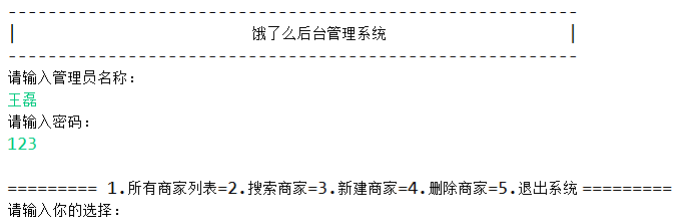
\includegraphics[width=12cm,height=5cm]{figures/jdbc1.png}
    \caption{管理员登录}
\end{figure}


2.菜单项一:所有商家列表

\begin{figure}[H]
    \centering
    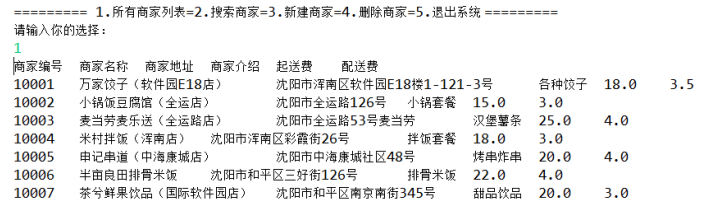
\includegraphics[width=15cm,height=5cm]{figures/jdbc2.png}
    \caption{商家列表}
\end{figure}

3.菜单项二:搜索商家

\begin{figure}[H]
    \centering
    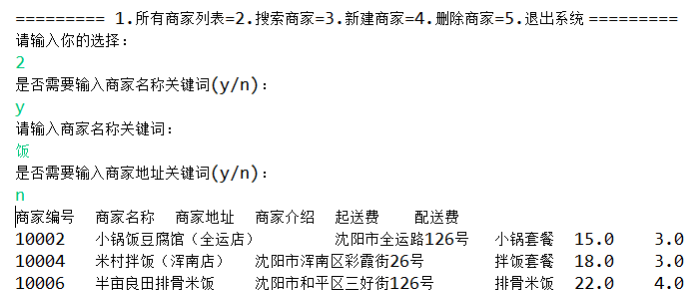
\includegraphics[width=15cm,height=7cm]{figures/jdbc3.png}
    \caption{搜索商家}
\end{figure}


4.菜单项三:新建商家

\begin{figure}[H]
    \centering
    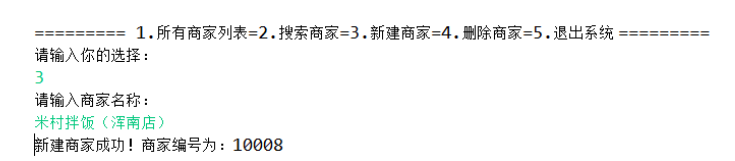
\includegraphics[width=15cm,height=4cm]{figures/jdbc4.png}
    \caption{新建商家}
\end{figure}

5.菜单项四:删除商家

\begin{figure}[H]
    \centering
    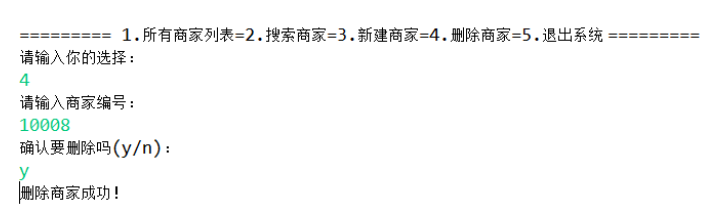
\includegraphics[width=15cm,height=5cm]{figures/jdbc5.png}
    \caption{删除商家}
\end{figure}

\subsection{商家入口}
1.商家登录,出现主菜单

\begin{figure}[H]
    \centering
    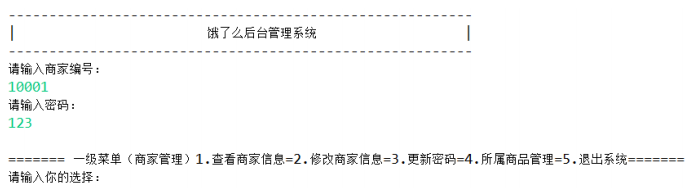
\includegraphics[width=15cm,height=5cm]{figures/jdbc6.png}
    \caption{商家登录}
\end{figure}

2.菜单项一:查看商家信息

\begin{figure}[H]
    \centering
    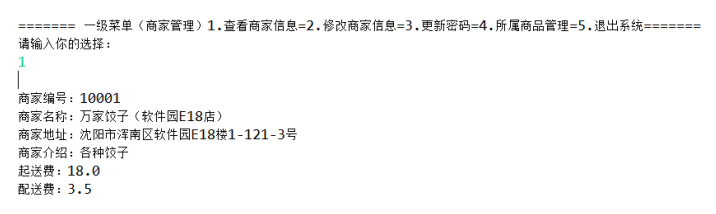
\includegraphics[width=15cm,height=5cm]{figures/jdbc7.png}
    \caption{查看商家信息}
\end{figure}

3.菜单项二:修改商家信息

\begin{figure}[H]
    \centering
    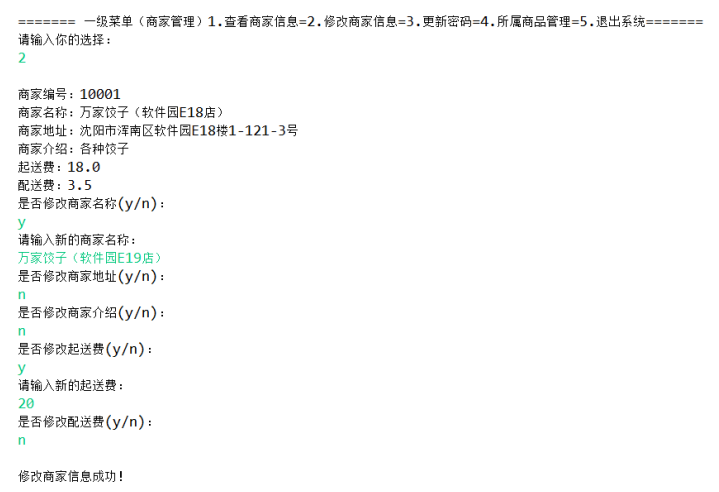
\includegraphics[width=15cm,height=12cm]{figures/jdbc8.png}
    \caption{修改商家信息}
\end{figure}

4.菜单项三:更新密码

\begin{figure}[H]
    \centering
    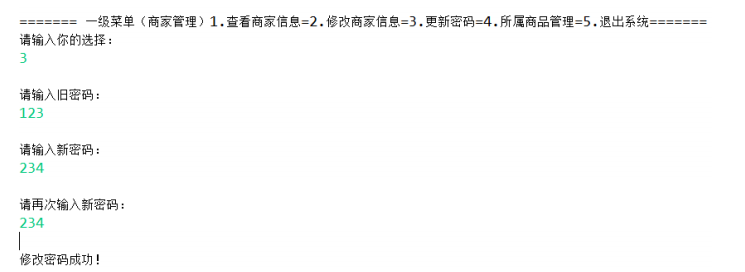
\includegraphics[width=15cm,height=7cm]{figures/jdbc9.png}
    \caption{更新密码}
\end{figure}~\\

5.菜单项四:所属商品管理(进入二级菜单,进行商品的增删改查管理)

\begin{figure}[H]
    \centering
    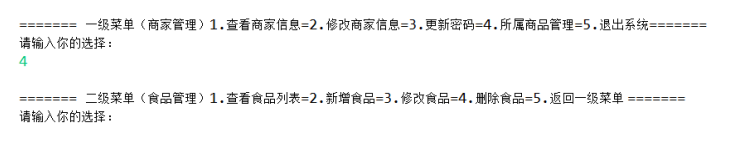
\includegraphics[width=15cm,height=4cm]{figures/jdbc10.png}
    \caption{更新密码}
\end{figure}


\subsection{商家二级菜单管理}
1.二级菜单项一:查看食品列表

\begin{figure}[H]
    \centering
    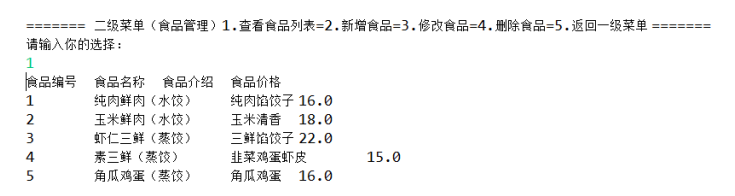
\includegraphics[width=15cm,height=4cm]{figures/jdbc11.png}
    \caption{查看食品列表}
\end{figure}

2.二级菜单项二:新增食品

\begin{figure}[H]
    \centering
    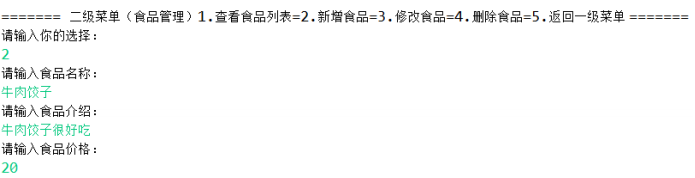
\includegraphics[width=15cm,height=4cm]{figures/jdbc12.png}
    \caption{新增食品}
\end{figure}

3.二级菜单项三:修改食品

\begin{figure}[H]
    \centering
    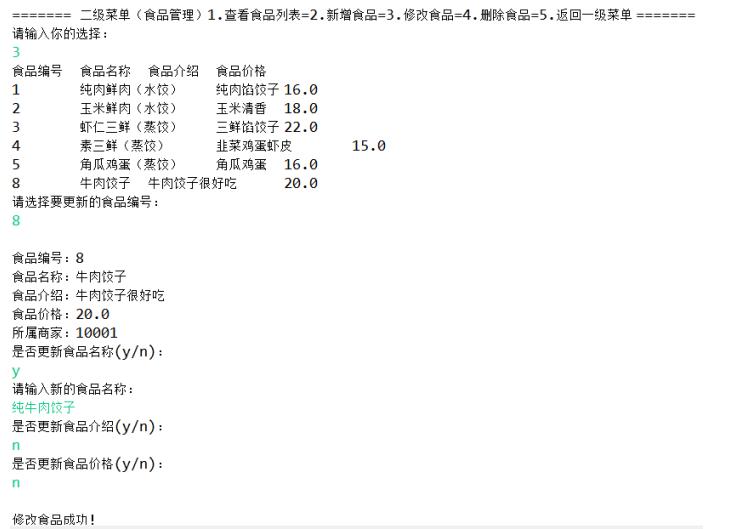
\includegraphics[width=15cm,height=12cm]{figures/jdbc13.png}
    \caption{修改食品}
\end{figure}


4.二级菜单项四:删除食品

\begin{figure}[H]
    \centering
    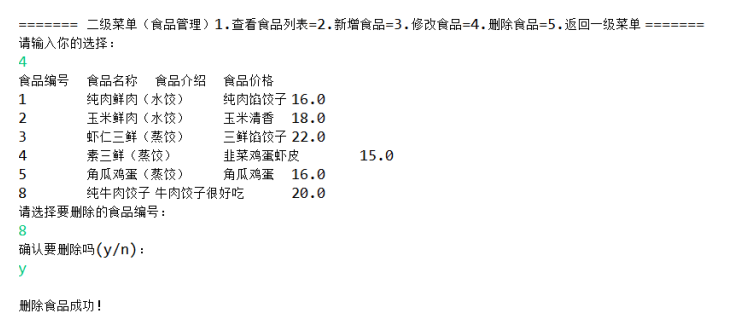
\includegraphics[width=15cm,height=8cm]{figures/jdbc14.png}
    \caption{删除食品}
\end{figure}


\section{项目设计}
\subsection{数据库设计}
本项目使用MYSQL数据库,选择DataGrip作为开发工具。在数据库的设计上,需要创建管理员、食品和商家共三张表。

\begin{figure}[H]
    \centering
    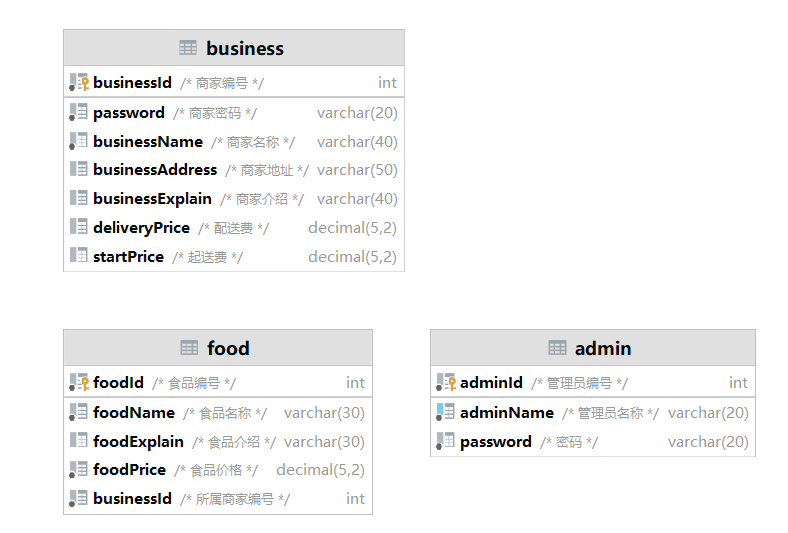
\includegraphics[width=15cm,height=10cm]{figures/table1.png}
    \caption{JDBC项目数据表}
\end{figure}

\subsection{后端设计}

\noindent
一. 开发环境

1. 开发工具:IDEA、DataGrip

2. 检查IDEA的jdk配置:jdk8


3. 检查IDEA的文件编码配置:utf-8

4. 检查MySQL配置:MySQL 8.0.30~\\


\noindent
二. 项目结构

本项目主要结构由上到下分为Entry层、view层、dao层:Entry即入口,包括商家和管理员两个入口,在入口接收到请求后调用view层,view层主要实现了一些对请求的进一步处理(例如询问是否按照地址查询),当请求明确之后,由view层调用dao层,dao层则是负责与数据库连接,对数据库进行操作。

除此之外的po文件夹里主要存放业务流中所需的持久对象,与数据表中的属性相对应,而util包中则存放一些常用的工具类。

\begin{figure}[H]
    \centering
    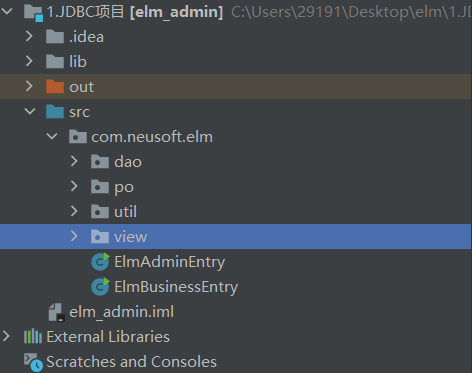
\includegraphics[width=15cm,height=13cm]{figures/structure1.png}
    \caption{项目结构}
\end{figure}

\section{功能优化}
在管理员或商家登陆成功后,输入数字选项阶段,如果输入数字以外的类型,程序会发生崩溃。我们针对此问题进行了优化,如果输入数字以外的类型,会提示“请输入正确格式的数字选项”。

\begin{figure}[H]
    \centering
    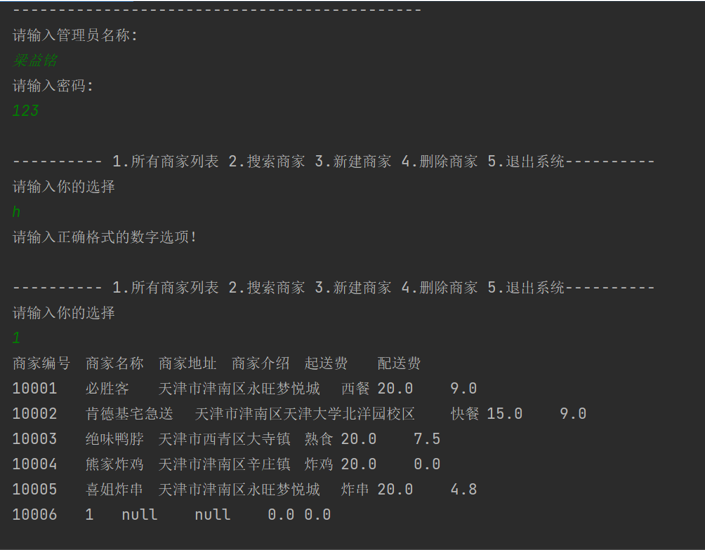
\includegraphics[width=15cm,height=12cm]{figures/improve1.png}
    \caption{项目一优化}
\end{figure}

